\subsection{Forecast Accuracy and the Baseline Comparison}
Table~\ref{tab:original_forecast} preserves the original run. On Antarex, LSTM RMSE was 1.216 pp against ARIMA's 1.516 pp, a 19.8\% reduction, while MAE changed only from 0.363 to 0.358 pp. The larger RMSE improvement indicates a stronger effect on large errors than on average absolute error. Across Westermo, the original LSTM reduced RMSE but ARIMA had lower MAE: no method wins under every loss.

The selected Antarex ARIMA$(3,1,0)$ coefficients are approximately $-0.011$, $-0.010$ and $-0.011$. With no drift, forecast increments quickly become small, making its predictions close to persistence; their RMSEs differ by only 0.000196 pp. Linear extrapolation performs worse in all four recordings, consistent with transient slopes not continuing through the forecast horizon. Figure~\ref{fig:forecast} shows the fixed original example interval; full-test scores, rather than that interval, support the comparisons.


\begin{table}[htbp]
\caption{Original test forecast errors: MAE / RMSE, in percentage points (pp) of total RAM. A uses 60 s; W1--W3 use 300 s. LSTM is the single Colab seed-42 run.}
\label{tab:original_forecast}
\centering\small
\setlength{\tabcolsep}{4pt}
\begin{tabular}{@{}lrrrr@{}}
\toprule
Model & A & W1 & W2 & W3\\
\midrule
Persistence & 0.361 / 1.517 & 0.094 / 0.363 & 0.109 / 0.317 & 0.240 / 0.715\\
Linear trend & 0.377 / 1.744 & 0.145 / 0.376 & 0.144 / 0.348 & 0.329 / 0.818\\
ARIMA & 0.363 / 1.516 & 0.093 / 0.318 & 0.105 / 0.291 & 0.230 / 0.658\\
Original LSTM & 0.358 / 1.216 & 0.099 / 0.296 & 0.117 / 0.258 & 0.251 / 0.608\\
\bottomrule
\end{tabular}
\end{table}


\begin{figure}[htbp]
\centering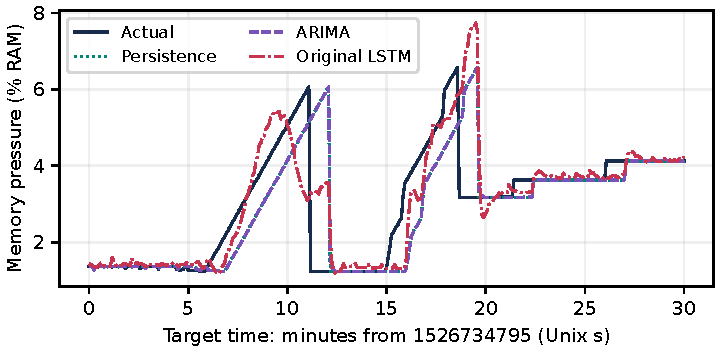
\includegraphics[width=\textwidth]{actual_predicted.pdf}
\Description{Actual and predicted memory pressure in percent of RAM over the fixed original first thirty minutes of Antarex test target times.}
\caption{Original Antarex 60-second-ahead rolling forecasts, aligned by target time. Predictions shown at a time were issued 60 s earlier. Persistence and ARIMA nearly overlap. This is the first fixed 30-minute test interval, not a best-case selection.}
\label{fig:forecast}
\end{figure}

\subsection{Random Seeds and the Memory-Only Ablation}
The new CPU runs use Python 3.12.14, PyTorch 2.8.0+cpu and two Torch threads. Table~\ref{tab:ablation} keeps them separate from Colab. On Antarex, multivariate mean RMSE is 1.204 pp versus memory-only 1.221 pp. Paired multivariate RMSE is lower in four of five Antarex seeds and all five W1 seeds, but only one W2 seed and no W3 seed. On W2 and W3, extra inputs also increase MAE in every paired seed. Additional telemetry therefore does not consistently improve this fixed model and training budget. The experiment does not isolate which feature helps or harms.

Both LSTM variants have lower mean RMSE than restricted ARIMA on each recording, but all their mean MAEs exceed ARIMA's. Training minimizes squared error, which weights large deviations strongly; lower RMSE with worse MAE is therefore possible. Seed SD describes optimization variability on these recordings, not a confidence interval for other systems. No additional labeled dataset or independent holdout was introduced.


\begin{table}[htbp]
\caption{Five-seed LSTM test errors: mean $\pm$ sample SD, in pp. Mem: memory-only; Multi: retained multivariate inputs. All five seeds are included.}
\label{tab:ablation}
\centering\small
\setlength{\tabcolsep}{4pt}
\begin{tabular}{@{}lrrrr@{}}
\toprule
Recording & MAE (Mem) & MAE (Multi) & RMSE (Mem) & RMSE (Multi)\\
\midrule
A & $0.378\pm0.018$ & $0.365\pm0.024$ & $1.221\pm0.015$ & $1.204\pm0.020$\\
W1 & $0.099\pm0.008$ & $0.103\pm0.008$ & $0.300\pm0.001$ & $0.297\pm0.002$\\
W2 & $0.110\pm0.005$ & $0.121\pm0.004$ & $0.260\pm0.003$ & $0.263\pm0.003$\\
W3 & $0.242\pm0.011$ & $0.278\pm0.026$ & $0.606\pm0.005$ & $0.618\pm0.009$\\
\bottomrule
\end{tabular}
\end{table}


\subsection{Warnings, Missed Events and Recognition Delay}
There are 1933 leak-active origins among 31,032 Antarex test origins and 35 fully covered injected events. Table~\ref{tab:original_warning} shows that the original LSTM warning improves precision and reduces false alarm starts from 86 to 42, but covers less leak-active time and misses one event. False alarm rates are 2.128/h for trend-only and 1.039/h for LSTM; false-positive exposure is 34.17 and 13.50 min respectively. Their detected-event 90th-percentile delays are 56.0 and 45.7 s. The disabled ARIMA rule is equivalent to always-off and misses all events.

The difference follows from the warning objective. Regression rewards accurate future levels over all origins, whereas the assisted rule demands both observed and forecast growth above a threshold for three readings. A model can predict the level closely while predicting insufficient continued growth. The additional condition suppresses some false alarms and some true warnings; minimizing forecast RMSE does not optimize event recall or warning F1.


\begin{table}[htbp]
\caption{Original Antarex test warnings. P/R: timestamp precision/recall; FA: false alarm starts; missed: events missed out of 35; delay: median seconds after injection among detected events only. A dash means undefined.}
\label{tab:original_warning}
\centering\small
\setlength{\tabcolsep}{4pt}
\begin{tabular}{@{}lrrrrrr@{}}
\toprule
Rule & P & R & F1 & FA & Missed & Delay (s)\\
\midrule
Trend only & 0.802 & 0.859 & 0.830 & 86 & 0 & 30\\
LSTM + trend & 0.848 & 0.466 & 0.601 & 42 & 1 & 31\\
ARIMA (off) & -- & 0.000 & 0.000 & 0 & 35 & --\\
\bottomrule
\end{tabular}
\end{table}


Event 1534, a low-intensity injection starting at 22:00:14 UTC on 19 May 2018, demonstrates this mechanism (Fig.~\ref{fig:missed}). During its 236 s and 47 eligible origins, forecast growth peaks at 0.216 pp/min, below the 0.4 threshold. Thus no reading can satisfy the forecast gate, irrespective of the three-reading requirement. Observed growth reaches 0.938 pp/min; trend-only warns after 56 s. Memory pressure spans approximately 3.20--7.17\%. The recorded scores explain the decision failure, not its allocation-level cause.

\begin{figure}[!htbp]
\centering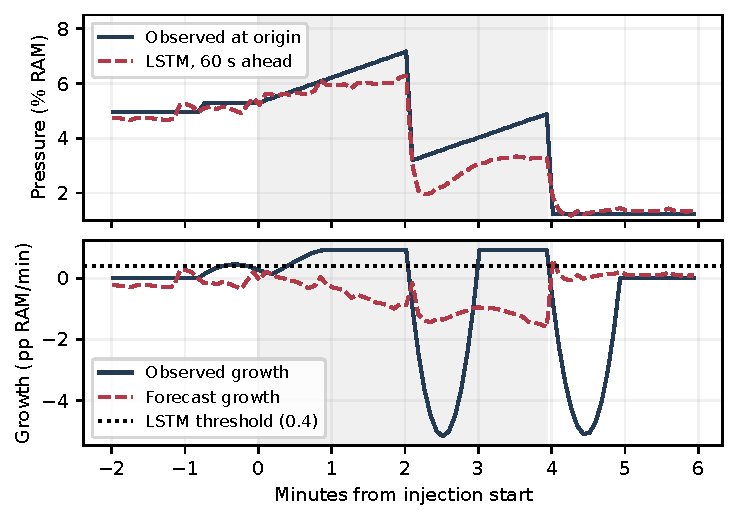
\includegraphics[width=\textwidth]{missed_event.pdf}
\Description{Two panels show memory pressure and growth scores around the original missed injection. Forecast growth stays below the warning threshold during the shaded interval.}
\caption{Original missed injected event 1534. Shading marks the recorded injection. Top: current pressure and the forecast issued at the same origin (its target is 60 s later). Bottom: observed and forecast growth; predicted growth remains below the LSTM gate throughout the injection. pp: percentage points of RAM.}
\label{fig:missed}
\end{figure}

The seed study weakens a general claim of fewer false alarms (Table~\ref{tab:repeat_warning}). Multivariate precision is $0.758\pm0.112$ and recall $0.461\pm0.010$; memory-only gives $0.648\pm0.071$ and $0.482\pm0.021$. Multivariate false starts range from 43 to 137, compared with the unchanged trend count of 86; memory-only ranges from 126 to 168. Each variant misses zero to two events depending on seed. Trend-only F1 remains 0.830, above every new LSTM-assisted run. The original precision/false-alarm advantage is therefore not stable across all repetitions. Validation selects thresholds separately for each run; forecast training variability and threshold decisions both influence these results.


\begin{table}[htbp]
\caption{Repeated LSTM-assisted Antarex warnings. F1 and FA/h are mean $\pm$ SD; missed is the range out of 35 events. Delay summarizes the five detected-event medians, not pooled events.}
\label{tab:repeat_warning}
\centering\small
\setlength{\tabcolsep}{4pt}
\begin{tabular}{@{}lrrrr@{}}
\toprule
Inputs & F1 & FA/h & Missed & Delay (s)\\
\midrule
Multivariate & $0.571\pm0.031$ & $2.014\pm1.052$ & 0--2 & $26.6\pm3.4$\\
Memory-only & $0.551\pm0.028$ & $3.405\pm0.449$ & 0--2 & $30.4\pm2.7$\\
\bottomrule
\end{tabular}
\end{table}


\subsection{Prototype Checks and Measurement Limits}
All 40 implementation tests passed, including loopback HTTP endpoints. Startup verified 76 source files covering 69,559 test origins. In a separate in-process benchmark on Windows with 8 logical CPUs and 7.8 GiB RAM, each recording received 100 replay/JSON requests and 100 warm model requests. Median replay times ranged from 7.05 to 21.84 ms; median warm inference ranged from 0.45 to 0.56 ms (95th percentiles 0.69--0.96 ms). All 404 first/warm inferences matched archived predictions within $10^{-6}$ pressure fraction. The first request, including library/model loading, took 5.34 s. Process resident memory increased from 25.4 to 402.3 MiB; this includes replay data, libraries and four models, not isolated monitoring overhead.

These measurements exclude HTTP transport and browser rendering. The live collector returned a Windows performance-counter error before any samples were recorded. No live timing, CPU-overhead or labeled live-detection result is reported. Longer live trials, missing-counter resilience and controlled overhead measurements remain unvalidated. The optional live mode uses exploratory trend warnings, not the archived Linux LSTM.
